\section{추후 연구}

\subsection{실험 환경 조성}
조파기와 관련하여 여전히 많은 매개 변수와 조작 변인이 존재한다. $N$은 바꿔볼 수도 있으며 모터 드라이버의 전류나 스텝 개수를 바꿔가며 더욱 섬세한 파를 생성할 수도 있다. 이는 실험적으로 접근해야하며 시간적 제약으로 인해 제작 및 기본 실험($A,~\omega$에 따른 파 조사)만 진행하였으나 조파기에 대한 더 나은 이해가 가능하다. 파고계의 위치를 바꿔가면서 조파기와의 거리에 따른 감쇠 효과에 대해 알아볼 수도 있다.

또, 소파기에 대한 연구를 진행할 수도 있는데 현재는 바구니에 수세미를 담은 다공성 구조로 수조의 양 말단에 두었으나 이를 3D 프린터로 정형화시켜 구멍의 크기나 배치 등에 따른 소파 효과를 확인할 수도 있다. 참고문헌에 의하면 다공성 구조가 아닌 일반 벽과 같은 소파기는 표면이 포물면일 때 제일 소파 효과가 크다고 한다.


%참고문헌 필요함.

\subsection{불규칙 파 생성}
조파기의 기본적인 목표는 축소 모형 실험에서 이에 맞는 환경을 조성해주는 것으로써 불규칙 파를 생성할 수 있어야 한다. 그 방법으로는 크게 조파판을 바꾸는 방법과 파 생성함수를 바꾸는 방법이 있다. 조파판을 바꾸는 것은 일체형으로 움직이는 조파판을 여러 요소로 나누어 다르게 움직이도록 하는 것이다.

\begin{figure}[htbp]
    \centering
    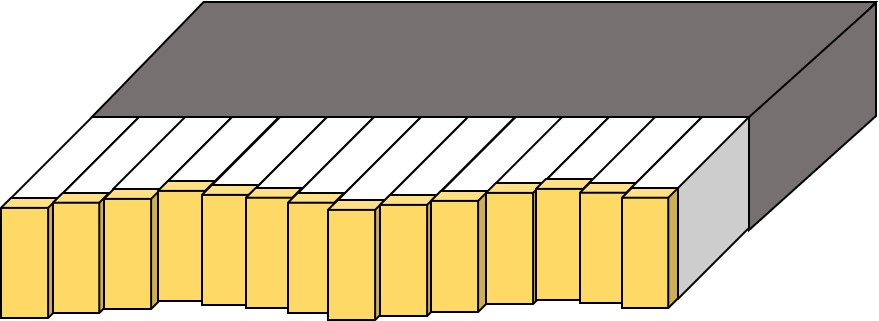
\includegraphics[width=10cm]{images/Wave_Maker(Snake).jpg}
    \caption{3차원 piston형 조파기}
    \label{Snake Wave Maker}
\end{figure}

%사진이 필요함.
이는 3차원 조파 수조로의 확장을 의미하며 조파판을 각 요소로 나누는 것이 유의미하려면 수조가 길고 좁은 것이 아닌 넓은 정사각형 모양이어야 한다. 하지만 이는 공간적 제약이 있으며 물을 여러 요소가 밀어내어 snake-like-wave를 발생시킬 수 있다. 현재는 sin파만 생성시켰으나 불규칙 파를 생성하는 것이 조파기의 궁극적인 목표이다. 그러려면 조파기가 piston형이라고 하더라도 판이 여러 조각으로 갈라져 각 조각마다 piston에 달려 있어야 하고 그만큼 많은 개수의 모터가 필요하며 아예 구동 방식을 달리 할 수도 있다.